%!TEX TS-program = xelatex
%!TEX options = -aux-directory=Debug -shell-escape -file-line-error -interaction=nonstopmode -halt-on-error -synctex=1 "%DOC%"
\documentclass{article}
\input{LaTeX-Submodule/template.tex}

% Additional packages & macros
\usepackage{subcaption}

% Header and footer
\newcommand{\unitName}{Computational Mathematics 2}
\newcommand{\unitTime}{Semester 1, 2024}
\newcommand{\unitCoordinator}{Dr Elliot Carr}
\newcommand{\documentAuthors}{Tarang Janawalkar}

\fancyhead[L]{\unitName}
\fancyhead[R]{\leftmark}
\fancyfoot[C]{\thepage}

% Copyright
\usepackage[
    type={CC},
    modifier={by-nc-sa},
    version={4.0},
    imagewidth={5em},
    hyphenation={raggedright}
]{doclicense}

\date{}

\begin{document}
%
\begin{titlepage}
    \vspace*{\fill}
    \begin{center}
        \LARGE{\textbf{\unitName}} \\[0.1in]
        \normalsize{\unitTime} \\[0.2in]
        \normalsize\textit{\unitCoordinator} \\[0.2in]
        \documentAuthors
    \end{center}
    \vspace*{\fill}
    \doclicenseThis
    \thispagestyle{empty}
\end{titlepage}
\newpage
%
\tableofcontents
\newpage
%
\section{The Transport Equation}
\subsection{Transport Phenomena}
Transport phenomena broadly comprises three disciplines; fluid
dynamics, heat transfer, and mass transfer.\ \textbf{Fluid dynamics} is
the study of the motion of fluids, including liquids and gases.\
\textbf{Heat transfer} is the study of how heat (thermal energy) is
transported, generated, dissipated, and/or converted in a physical
system.\ \textbf{Mass transfer} is the study of the movement of mass
from one location to another.

The mathematical equations used to describe the above phenomena involve
three fundamental mechanisms of transport:
\begin{enumerate}
    \item Diffusion
    \item Advection
    \item Reaction
\end{enumerate}
\subsubsection{Diffusion}
\textit{Diffusion} is the gradual movement of a substance from regions of high
concentration to regions of low concentration. The direction of
diffusion is determined by the sign of the negative gradient of the
concentration.
\subsubsection{Advection}
\textit{Advection} is the transport of a substance by bulk motion of a fluid.
Advection is driven by a vector field in which the substance is
transported.
\subsubsection{Reaction}
Reaction is the process in which substances are created or destroyed.
Reaction is represented as a source or sink function.
\subsection{Transport Equation}
The general form of the transport equation is given by
\begin{equation*}
    \underbrace{\pdv{u}{t}}_{\text{unsteady term}} + \underbrace{\symbf{\nabla} \cdot \left( \symbf{v} u \right) \vphantom{\pdv{u}{t}}}_{\text{advection term}} = \underbrace{\symbf{\nabla} \cdot \left( \symbf{D} \symbf{\nabla} u \right) \vphantom{\pdv{u}{t}}}_{\text{diffusion term}} + \underbrace{R \vphantom{\pdv{u}{t}}}_{\text{reaction term}}
\end{equation*}
where \(u\left( \symbf{x},\: t \right)\) is the quantity being transported
at position \(\symbf{x}\) and time \(t\), \(\symbf{v}\left( \symbf{x},\: t \right) \in \R^n\)
is a velocity vector field which drives \(u\),
\(\symbf{D} \in \R^{n \times n}\) is the diffusion matrix, and \(R\) is
a reaction term.\ \(n\) represents the dimension of the spatial domain
of the problem, which can be 1, 2, or 3.

An alternative form of the transport equation combines the divergence
terms
\begin{equation*}
    \underbrace{\pdv{u}{t} \vphantom{\pdv{u}{t}}}_{\text{unsteady term}} + \underbrace{\symbf{\nabla} \cdot \symbf{q} \vphantom{\pdv{u}{t}}}_{\text{flux term}} = \underbrace{R \vphantom{\pdv{u}{t}}}_{\text{reaction term}}
\end{equation*}
where \(\symbf{q} = \symbf{v} u - \symbf{D} \symbf{\nabla} u\) is the
\textit{flux vector}.
\subsubsection{Domain}
This PDE is defined on a specified domain \(\Omega\) which is an open
connected subset of \(\R^n\), with the boundary \(\partial \Omega\).
\subsubsection{Derivation}
The transport equation can be derived from the conservation of mass
principle: the rate of change of the quantity \(u\) within a region
\(D\) must be balanced by the net flow of \(u\) in/out of the boundary
\(\partial{D}\) of \(D\), and the rate of creation or destruction of
\(u\) within \(D\). Consider an arbitrarily small sub-domain \(D\) of
\(\Omega\) with boundary \(\partial D\), then:
\begin{align*}
    \biggl\{ \parbox[c]{2.5cm}{\centering Rate of change                                                                                                          \\ of \(u\) in \(D\)} \biggr\} & =
    -\biggl\{ \parbox[c]{2cm}{\centering \(u\) leaving \(D\)                                                                                                      \\ across \(\partial{D}\)} \biggr\}
    + \biggl\{ \parbox[c]{4cm}{\centering Generation/Destruction                                                                                                  \\of \(u\) within \(D\)} \biggr\} \\
    \odv{}{t} \int_D u \odif{V}                                                    & = -\int_{\partial{D}} \symbf{q} \cdot \symbf{n} \odif{s} + \int_D R \odif{V} \\
    \int_D \pdv{u}{t} \odif{V}                                                     & = -\int_{D} \symbf{\nabla} \cdot \symbf{q} \odif{V} + \int_D R \odif{V}      \\
    \int_D \left( \pdv{u}{t} + \symbf{\nabla} \cdot \symbf{q} - R \right) \odif{V} & = 0                                                                          \\
    \pdv{u}{t} + \symbf{\nabla} \cdot \symbf{q}                                    & = R.
\end{align*}
\subsection{Special Cases}
\subsubsection{One Spatial Dimension}
In one spatial dimension, the transport equation reduces to
\begin{equation*}
    \pdv{u}{t} + \pdv{}{x} \left( v u \right) = \pdv{}{x} \left( D \pdv{u}{x} \right) + R.
\end{equation*}
where \(u\left( x,\: t \right)\) is a function of one spatial dimension
and time, \(v\) is the velocity, and \(D > 0\) is the diffusivity.
\subsubsection{Two Spatial Dimensions}
In two spatial dimensions, the transport equation reduces to
\begin{equation*}
    \pdv{u}{t} + \pdv{}{x} \left( v_x u \right) + \pdv{}{y} \left( v_y u \right) = \pdv{}{x} \left( D_{xx} \pdv{u}{x} \right) + \pdv{}{y} \left( D_{yy} \pdv{u}{y} \right) + R.
\end{equation*}
where \(u\left( x,\: y,\: t \right)\) is a function of two spatial
dimensions and time, \(v_x\) and \(v_y\) are the velocities in the \(x\)
and \(y\) directions, and \(D_{xx}\) and \(D_{yy}\) are the diffusivities
in the \(x\) and \(y\) directions.
\subsubsection{Eliminating Terms}
The transport equation is also called the
\textit{advection-diffusion-reaction equation}.
\begin{itemize}
    \item If the \textit{velocity term} \(\symbf{v}\) is the zero
          vector, the equation reduces to the
          \textit{diffusion-reaction equation}.
    \item If the \textit{diffusion term} \(\symbf{D}\) is the zero
          matrix, the equation reduces to the
          \textit{advection-reaction equation}.
    \item If the \textit{reaction term} \(R\) is zero, the equation
          reduces to the \textit{advection-diffusion equation}.
\end{itemize}
\subsection{Classification}
While the terms in the transport equation may be constant or variable,
certain combinations of these terms lead to different solution methods.
\begin{itemize}
    \item The velocity vector \(\symbf{v}\) may be a constant vector or
          a function of space \(\symbf{x}\), time \(t\), and/or the
          solution \(u\).
    \item The diffusion matrix \(\symbf{D}\) may be a constant matrix
          or a function of space \(\symbf{x}\), time \(t\), and/or the
          solution \(u\).
    \item The reaction term \(R\) may be a constant or a function of
          space \(\symbf{x}\), time \(t\), and/or the solution \(u\).
\end{itemize}
When \(\symbf{v}\) and \(\symbf{D}\) are \underline{not} functions of \(u\), and
\(R\) is a \underline{linear} function of \(u\), the transport equation is
called \textit{linear}. The equation is \textit{nonlinear} otherwise.
The domain \(\Omega\) is called \textit{heterogeneous} if any of the
coefficients \(\symbf{v}\), \(\symbf{D}\), or \(R\) are functions of
space \(\symbf{x}\), and \textit{homogeneous} otherwise.
\subsection{Dimensional Analysis}
Performing a dimensional analysis on the transport equation allows us
to associate physical units with the coefficients of the equation. This
analysis is useful for verifying the correctness of the equation and
for scaling the equation to a dimensionless form. The terms in the
equation
\begin{equation*}
    \pdv{u}{t} + \symbf{\nabla} \cdot \left( \symbf{v} u \right) = \symbf{\nabla} \cdot \left( \symbf{D} \symbf{\nabla} u \right) + R
\end{equation*}
may only be added or subtracted if they have the same units. Therefore,
given that
\begin{equation*}
    \left[ \pdv{u}{t} \right] \equiv \frac{\left[ u \right]}{\left[ t \right]} = \frac{\left[ u \right]}{\mathsf{T}}
\end{equation*}
we can deduce the units of other terms in the equation.
\begin{align*}
    \left[ \symbf{\nabla} \cdot \left( \symbf{v} u \right) \right] \equiv \frac{\left[ \symbf{v} \right] \left[ u \right]}{\left[ x \right]} = \frac{\left[ u \right]}{\mathsf{T}}                                                                                                        & \implies \left[ \symbf{v} \right] = \frac{\mathsf{L}}{\mathsf{T}}   \\
    \left[ \symbf{\nabla} \cdot \left( \symbf{D} \symbf{\nabla} u \right) \right] \equiv \frac{\left[ \symbf{D} \right] \left[ \symbf{\nabla} u \right]}{\left[ x \right]} = \frac{\left[ \symbf{D} \right] \left[ u \right]}{{\left[ x \right]}^2} = \frac{\left[ u \right]}{\mathsf{T}} & \implies \left[ \symbf{D} \right] = \frac{\mathsf{L}^2}{\mathsf{T}} \\
    \left[ R \right] \equiv \frac{\left[ u \right]}{\left[ t \right]}                                                                                                                                                                                                                     & \implies \left[ R \right] = \frac{\left[ u \right]}{\mathsf{T}}
\end{align*}
\subsection{Initial and Boundary Conditions}
In addition to the transport equation, which describes the behaviour of
\(u\) within the domain \(\Omega\), the problem must also specify how
\(u\) behaves at the boundary \(\partial \Omega\) with \textit{boundary
conditions}. Some common boundary conditions include:
\begin{itemize}
    \item Specified value: \(u\left( \symbf{x},\: t \right) = u_b\) on
          \(\partial \Omega\)
    \item Specified flux: \(\symbf{q} \cdot \symbf{n} = q_b\) on
          \(\partial \Omega\)
    \item Specified gradient: \(\symbf{\nabla} u \cdot \symbf{n} =
          d_b\) on \(\partial \Omega\)
\end{itemize}
Here \(u_b\), \(q_b\), and \(d_b\) may be constants or scalar functions
of \(\symbf{x}\) and/or \(t\), and \(\symbf{n}\) is the unit normal vector
to \(\partial \Omega\), directed outward from \(\Omega\).

We may also wish to use a Robin condition to describe a general
boundary condition of the form:
\begin{equation*}
    a u + b \left( \symbf{\nabla} u \cdot \symbf{n} \right) = c
\end{equation*}
where \(a\), \(b\), and \(c\) are constants or scalar functions of
\(\symbf{x}\) and/or \(t\). When \(c = 0\), the condition is called
\textit{homogeneous}, and \textit{nonhomogeneous} otherwise.

In addition to these conditions, an \textit{initial condition} is
required to specify the profile of \(u\) at time \(t = 0\).
\subsection{Steady-State Problems}
If it exists, the \textit{steady-state solution} of the transport
equation is the solution of the equation when the time-derivative of
\(u\) is zero:
\begin{equation*}
    \pdv{u}{t} = 0.
\end{equation*}
The steady-state solution is useful for understanding the long-term
behaviour of the system, where it is assumed that the system is no longer
time-dependent. The steady-state solution is expressed as
\(u_\infty = \lim_{t \to \infty} u\left( \symbf{x},\: t \right)\).
\section{Finite Volume Method}
The \textit{Finite Volume Method} (FVM) is a method for solving the
transport equation at discrete points (nodes) in space: \(u_i\left( t
\right) \approx u\left( \symbf{x}_i,\: t \right)\) for \(i = 1,\: 2,\:
\ldots,\: N\). FVM is a \textit{spatial discretisation} method that
converts a spatially-continuous initial-boundary value problem to a
satially-discrete initial-value problem.

The FVM is used in transport phenomena because the approximate solution
obeys the laws of conservation of mass and energy. This is generally
not true for finite differences or finite element methods. FVM also has
the advantage of being able to handle complex geometries and irregular
grids.
\subsection{Discretising the Domain}
The basic geometric structure used in the FVM is called the
\textbf{mesh}. A mesh is a partitioning of the domain \(\Omega\) into
smaller sub-domains called \textbf{elements}. The intersection of edges
in this mesh are called \textbf{vertices}. An example of a 1D mesh is
shown below.
\begin{figure}[H]
    \centering
    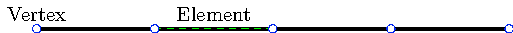
\includegraphics[width = 0.8\linewidth]{figures/1d-mesh.pdf}
    \caption{1D mesh.} % \label{}
\end{figure}
In two and three dimensions, the mesh may be either \textit{structured}
or \textit{unstructured} as shown below. Unstructured meshes typically
consist of triangles (or tetrahedra in 3D).
\begin{figure}[H]
    \centering
    \begin{subfigure}[t]{0.45\textwidth}
        \centering
        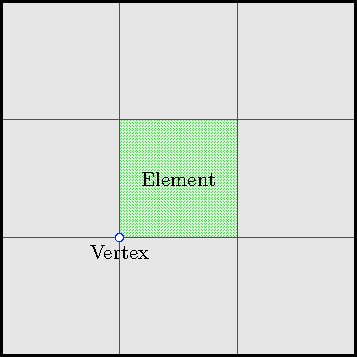
\includegraphics[height = 4cm]{figures/2d-structured-mesh.pdf}
        \caption{2D structured mesh.} % \label{}
    \end{subfigure}
    %
    \begin{subfigure}[t]{0.45\textwidth}
        \centering
        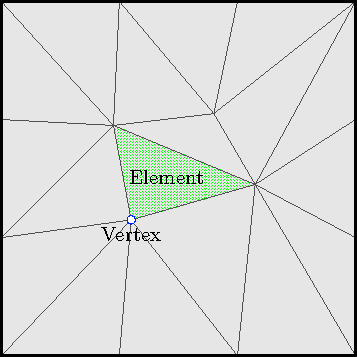
\includegraphics[height = 4cm]{figures/2d-unstructured-mesh.pdf}
        \caption{2D unstructured mesh.} % \label{}
    \end{subfigure}
\end{figure}
The FVM defines:
\begin{itemize}
    \item \textbf{Nodes} \(\symbf{x}_i\), at which the solution is
          approximated by \(u_i\)
    \item \textbf{Control volumes} \(\Omega_i\), over which the
          conservation principle is applied
\end{itemize}
where \(i = 1,\: 2,\: \ldots,\: N\) is the index of the nodes.
There are several ways to define the control volumes. Two common
approaches are:
\begin{itemize}
    \item \textbf{Cell-Centred Control Volumes}: Nodes are positioned
          at the centroids of elements, and control volumes are defined over
          elements.
    \item \textbf{Vertex-Centred Control Volumes}: Nodes are positioned
          at vertices, and control volumes are constructed using the centroids
          of adjacent element boundaries.
\end{itemize}
This is illustrated in 1D and 2D in the following figures.
\begin{figure}[H]
    \centering
    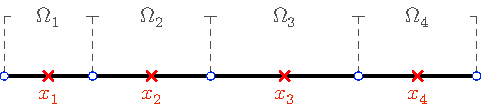
\includegraphics[width = 0.8\linewidth]{figures/1d-cell-centered.pdf}
    \caption{1D mesh with cell-centred control volumes.} % \label{}
\end{figure}
\begin{figure}[H]
    \centering
    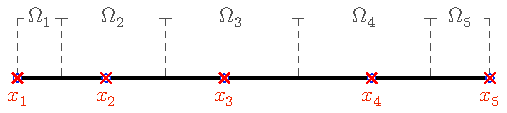
\includegraphics[width = 0.8\linewidth]{figures/1d-vertex-centered.pdf}
    \caption{1D mesh with vertex-centred control volumes.} % \label{}
\end{figure}
\begin{figure}[H]
    \centering
    \begin{subfigure}[t]{0.45\linewidth}
        \centering
        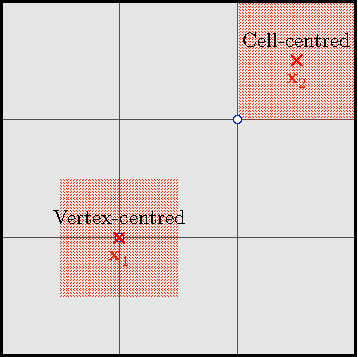
\includegraphics[height = 4cm]{figures/2d-structured-nodes.pdf}
        \caption{2D structured mesh with vertex-/cell- centred control volumes.} % \label{}
    \end{subfigure}
    \begin{subfigure}[t]{0.45\linewidth}
        \centering
        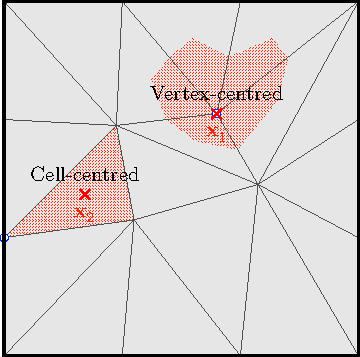
\includegraphics[height = 4cm]{figures/2d-unstructured-nodes.pdf}
        \caption{2D unstructured mesh with vertex-/cell- centred control volumes.} % \label{}
    \end{subfigure}
\end{figure}
For problems in three dimensions using structured meshes, control
volumes are cubes (or rectangular prisms). For unstructured meshes with
control volumes using the cell-centred approach, elements themselves are
used as control volumes. For the vertex-centred approach, control volume
boundaries are defined using the centroids of adjacent element boundaries.
\subsection{General Strategy}
Consider a mesh with \(N\) nodes and \(N\) control volumes:
\begin{enumerate}
    \item Label the nodes \(x_1,\: x_2,\: \ldots,\: x_N\) and the
          unknowns \(u_1,\: u_2,\: \ldots,\: u_N\).
    \item Identify the control volume types (interior node, boundary
          node).
    \item Integrate the transport equation over each control volume and
          apply the Divergence theorem to the flux term.
    \item Incorporate the boundary conditions to approximate/discretise
          all remaining terms.
\end{enumerate}
To discretise the transport equation, let us integrate the transport
equation over each control volume \(\Omega_i\):
\begin{align*}
    \pdv{u}{t} + \symbf{\nabla} \cdot \symbf{q}                                                                  & = R                          \\
    \int_{\Omega_i} \pdv{u}{t} \odif{V} + \int_{\Omega_i} \left( \symbf{\nabla} \cdot \symbf{q} \right) \odif{V} & = \int_{\Omega_i} R \odif{V}
\end{align*}
Applying the divergence theorem to the flux term, we have
\begin{equation*}
    \odv*{\int_{\Omega_i} u \odif{V}}{t} + \int_{\partial \Omega_i} \left( \symbf{q} \cdot \symbf{n} \right) \odif{s} = \int_{\Omega_i} R \odif{V}
\end{equation*}
where \(\partial \Omega_i\) is the control volume boundary of \(\Omega_i\),
and \(\symbf{n}\) is the outward unit vector normal to \(\partial \Omega_i\),
directed out of \(\Omega_i\). Consider the spatial average of \(u\) and
\(R\) over \(\Omega_i\):
\begin{equation*}
    \bar{u}_i = \frac{1}{V_i} \int_{\Omega_i} u \odif{V}, \qquad \bar{R}_i = \frac{1}{V_i} \int_{\Omega_i} R \odif{V}
\end{equation*}
where \(V_i\) is the volume of \(\Omega_i\). Using this quantity, we can
rewrite the transport equation as
\begin{equation*}
    \odv{\bar{u}_i}{t} + \frac{1}{V_i} \int_{\partial \Omega_i} \left( \symbf{q} \cdot \symbf{n} \right) \odif{s} = \bar{R}_i.
\end{equation*}
We can now approximate this ODE using the discrete approximations, \(u_i\)
and \(R_i\), at each node \(\symbf{x}_i\).
\begin{equation*}
    \odv{u_i}{t} = - \frac{1}{V_i} \int_{\partial \Omega_i} \left( \symbf{q} \cdot \symbf{n} \right) \odif{s} + R_i
\end{equation*}
\subsection{FVM in 1D}
Before we consider the 1D case for the FVM, let us define the following
geometric quantities (for the vertex-centred control volume strategy):
\begin{figure}[H]
    \centering
    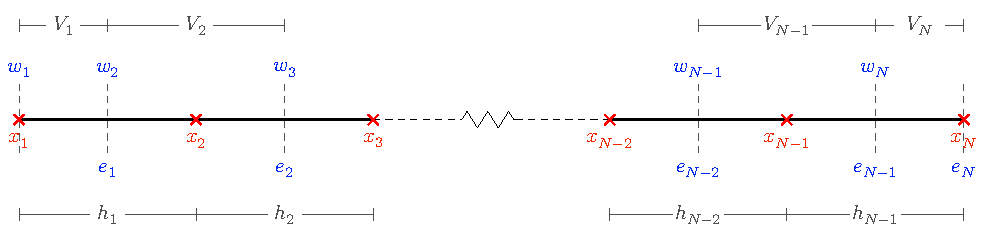
\includegraphics[width = \linewidth]{figures/1d-fvm.pdf}
    \caption{1D FVM.} % \label{}
\end{figure}
where
\begin{itemize}
    \item \(\Omega = \ointerval{x_1}{x_N}\)
    \item \(\Omega_i = \ointerval{w_i}{e_i}\) is the control volume for node \(i\)
    \item \(h_i\) is the spacing between nodes \(i\) and \(i + 1\)
          \begin{equation*}
              h_i = x_{i+1} - x_i \quad \text{for \(i = 1,\: \ldots,\: N-1\)}
          \end{equation*}
    \item \(V_i\) is the volume of control volume \(\Omega_i\)
          \begin{equation*}
              V_i =
              \begin{cases}
                  \displaystyle \frac{h_1}{2},           & i = 1                       \\
                  \displaystyle \frac{h_{i-1} + h_i}{2}, & 2 \leqslant i \leqslant N-1 \\
                  \displaystyle \frac{h_{N-1}}{2},       & i = N
              \end{cases}
          \end{equation*}
    \item \(w_i\) and \(e_i\) are the west and east boundaries of
          control volume \(\Omega_i\)
          \begin{align*}
              w_i & =
              \begin{cases}
                  \displaystyle x_1,                     & i = 1                     \\
                  \displaystyle \frac{x_{i-1} + x_i}{2}, & 2 \leqslant i \leqslant N
              \end{cases}
              \\
              e_i & =
              \begin{cases}
                  \displaystyle \frac{x_i + x_{i+1}}{2}, & 1 \leqslant i \leqslant N-1 \\
                  \displaystyle x_N,                     & i = N
              \end{cases}
          \end{align*}
\end{itemize}
Then, if we integrate over all control volumes \(\Omega_i\) in 1D, the
spatial averages simplify to:
\begin{equation*}
    \bar{u}_i = \frac{1}{V_i} \int_{w_i}^{e_i} u \odif{x}, \qquad \bar{R}_i = \frac{1}{V_i} \int_{w_i}^{e_i} R \odif{x}
\end{equation*}
likewise, the flux term becomes,
\begin{align*}
    \int_{\Omega_i} \left( \symbf{\nabla} \cdot \symbf{q} \right) \odif{V} & = \int_{w_i}^{e_i} \pdv{q}{x} \odif{x} \\
                                                                           & = q_{e_i} - q_{w_i}
\end{align*}
Then using the strategy outlined in the previous section, we find:
\begin{equation*}
    \odv{u_i}{t} = \frac{1}{V_i} \left( q_{w_i} - q_{e_i} \right) + R_i
\end{equation*}
where \(u_i \approx \bar{u}_i\) and \(R_i \approx \bar{R}_i\). This equation
can now be used to solve an initial-boundary value problem using the FVM.
This is done by applying the finite-difference method at internal nodes,
using:
\begin{align*}
    \pdv{u}{x}\left( w_i,\: t \right) & = \frac{u_i - u_{i-1}}{h_{i-1}} \\
    \pdv{u}{x}\left( e_i,\: t \right) & = \frac{u_{i+1} - u_i}{h_i}
\end{align*}
and at boundary nodes, using the boundary conditions:
\begin{align*}
    \pdv{u}{x}\left( w_1,\: t \right) & = \pdv{u}{x}\left( 0,\: t \right) & \pdv{u}{x}\left( e_1,\: t \right) & = \frac{u_2 - u_1}{h_1}           &  & \text{(left boundary)}  \\
    \pdv{u}{x}\left( w_N,\: t \right) & = \frac{u_N - u_{N-1}}{h_{N-1}}   & \pdv{u}{x}\left( e_N,\: t \right) & = \pdv{u}{x}\left( L,\: t \right) &  & \text{(right boundary)}
\end{align*}
we find a linear ODE of the form:
\begin{equation*}
    \odv{\symbf{u}}{t} = \symbf{A} \symbf{u} + \symbf{b}\left( t \right), \qquad \symbf{u}\left( 0 \right) = \symbf{u}^{\left( 0 \right)}
\end{equation*}
where \(\symbf{u} = {\left( u_1,\: \dots,\: u_N \right)}^\top\) is the
numerical solution vector at time \(t\) containing the solution at each
node \(x_i\) and \(\symbf{u}^{\left( 0 \right)} = {\left( f\left( x_1 \right),\: \dots,\: f\left( x_N \right) \right)}^\top\)
is the initial solution vector.

\(\symbf{A} \in \R^{N \times N}\) is a tridiagonal matrix containing
the coefficients of the finite-difference method, and
\(\symbf{b}\left( t \right)\) contains any time-dependent terms in the
transport equation. This ODE can be solved using standard ODE solving
techniques. When the transport equation is nonlinear, the RHS cannot
be written as a matrix-vector product, so that
\begin{equation*}
    \odv{\symbf{u}}{t} = \symbf{F}\left( t,\: \symbf{u}\left( t \right) \right).
\end{equation*}
\subsection{Time Discretisation}
The resulting ODE can be solved using a time-stepping method such as
the Forward Euler, the Backward Euler, or the Crank-Nicolson methods.
To solve this initial value problem, we will consider a sufficiently
large final time, \(T\), so that the problem is solved between \(t =
0\) and \(t = T\). Then, we will discretise the time domain into \(M\)
time steps of size \(\fdif{t} = T/M = t_{n+1} - t_n\), such that \(t_n
= n \fdif{t}\) for \(n = 0,\: 1,\: \ldots,\: M\).

Let us rewrite the ODE in the equivalent form:
\begin{equation*}
    \odv{\symbf{u}}{t} = \symbf{A} \symbf{u} + \symbf{b}_1 + \symbf{b}_2\left( t \right), \qquad \symbf{u}\left( 0 \right) = \symbf{u}^{\left( 0 \right)}
\end{equation*}
such that \(\symbf{b}_2\left( t \right) = {\left( R\left( x_1,\: t \right),\: \dots,\: R\left( x_N,\: t \right) \right)}^\top\)
is the time-dependent flux term, and \(\symbf{b}_1 = \symbf{b}\left( t \right) - \symbf{b}_2\left( t \right)\)
contains the time-independent reaction term. We will now compute
\(\symbf{u}^{\left( n \right)} = {\left( u_1^{\left( n \right)},\: \dots,\: u_N^{\left( n \right)} \right)}^\top\),
where \(u_i^{\left( n \right)} \approx u_i\left( t_n \right) = u\left( x_i,\: t_n \right)\),
is the solution at \(x = x_i\) and time \(t = t_n\), using the
\(\theta\)-method.

Let us first integrate the ODE over the time interval
\(\ointerval{t_n}{t_{n+1}}\):
\begin{align*}
    \int_{t_n}^{t_{n+1}} \odv{\symbf{u}}{t} \odif{t}              & = \int_{t_n}^{t_{n+1}} \left( \symbf{A} \symbf{u} + \symbf{b}_1 + \symbf{b}_2\left( t \right) \right) \odif{t}                                              \\
    \symbf{u}\left( t_{n+1} \right) - \symbf{u}\left( t_n \right) & = \symbf{A} \int_{t_n}^{t_{n+1}} \symbf{u} \odif{t} + \int_{t_n}^{t_{n+1}} \symbf{b}_1 \odif{t} + \int_{t_n}^{t_{n+1}} \symbf{b}_2\left( t \right) \odif{t} \\
    \symbf{u}^{\left( n+1 \right)} - \symbf{u}^{\left( n \right)} & = \symbf{A} \int_{t_n}^{t_{n+1}} \symbf{u} \odif{t} + \symbf{b}_1 \left( t_{n+1} - t_n \right) + \int_{t_n}^{t_{n+1}} \symbf{b}_2\left( t \right) \odif{t}
\end{align*}
To integrate the time-dependent terms, we will use the weighted \(\theta\)
approximation, where
\begin{equation*}
    \int_{t_n}^{t_{n+1}} f\left( t \right) \odif{t} \approx \fdif{t} \left[ \left( 1 - \theta \right) f\left( t_n \right) + \theta f\left( t_{n+1} \right) \right].
\end{equation*}
Therefore, we have
\begin{align*}
    \symbf{u}^{\left( n+1 \right)} - \symbf{u}^{\left( n \right)}                               & = \fdif{t} \symbf{A} \left[ \left( 1 - \theta_1 \right) \symbf{u}^{\left( n \right)} + \theta_1 \symbf{u}^{\left( n+1 \right)} \right] + \symbf{b}_1 \fdif{t} + \fdif{t} \left[ \left( 1 - \theta_2 \right) \symbf{b}_2^{\left( n \right)} + \theta_2 \symbf{b}_2^{\left( n+1 \right)} \right] \\
    \symbf{u}^{\left( n+1 \right)} - \symbf{A} \theta_1 \fdif{t} \symbf{u}^{\left( n+1 \right)} & = \symbf{u}^{\left( n \right)} + \fdif{t} \left( 1 - \theta_1 \right) \symbf{A} \symbf{u}^{\left( n \right)} + \fdif{t} \symbf{b}_1 + \fdif{t} \left[ \left( 1 - \theta_2 \right) \symbf{b}_2^{\left( n \right)} + \theta_2 \symbf{b}_2^{\left( n+1 \right)} \right]                           \\
    \left( \symbf{I} - \fdif{t} \theta_1 \symbf{A} \right) \symbf{u}^{\left( n+1 \right)}       & = \left[ \symbf{I} + \fdif{t} \left( 1 - \theta_1 \right) \symbf{A} \right] \symbf{u}^{\left( n \right)} + \fdif{t} \left[ \symbf{b}_1 + \left( 1 - \theta_2 \right) \symbf{b}_2^{\left( n \right)} + \theta_2 \symbf{b}_2^{\left( n+1 \right)} \right] \\
    \tilde{\symbf{A}} \symbf{u}^{\left( n+1 \right)}                                              & = \tilde{\symbf{b}}
\end{align*}
for two choices of \(\theta_1\) and \(\theta_2\).
Setting \(\theta_1 = \theta_2 = 0\), we obtain the Forward Euler method:
\begin{equation*}
    \symbf{u}^{\left( n+1 \right)} = \left( \symbf{I} + \fdif{t} \symbf{A} \right) \symbf{u}^{\left( n \right)} + \fdif{t} \left( \symbf{b}_1 + \symbf{b}_2^{\left( n \right)} \right)
\end{equation*}
which is an explicit method. Setting \(\theta_1 = \theta_2 = 1\), yields
the Backward Euler method:
\begin{equation*}
    \left( \symbf{I} - \fdif{t} \symbf{A} \right) \symbf{u}^{\left( n+1 \right)} = \symbf{u}^{\left( n \right)} + \fdif{t} \left( \symbf{b}_1 + \symbf{b}_2^{\left( n+1 \right)} \right)
\end{equation*}
while setting \(\theta_1 = \theta_2 = \frac{1}{2}\) gives the Crank-Nicolson
method:
\begin{equation*}
    \left( \symbf{I} - \frac{\fdif{t}}{2} \symbf{A} \right) \symbf{u}^{\left( n+1 \right)} = \left( \symbf{I} + \frac{\fdif{t}}{2} \symbf{A} \right) \symbf{u}^{\left( n \right)} + \frac{\fdif{t}}{2} \left( 2 \symbf{b}_1 + \symbf{b}_2^{\left( n \right)} + \symbf{b}_2^{\left( n+1 \right)} \right)
\end{equation*}
which are both implicit methods. Using different values for \(\theta_1\)
and \(\theta_2\) is also possible, and is called the IMEX method (Implicit-Explicit).
\subsection{Time Discretisation for the 1D FVM}
We can apply the same time discretisation to the 1D FVM. Let us
consider the 1D FVM with the following ODE:
\begin{equation*}
    \odv{u_i}{t} = \frac{1}{V_i} \left( q_{w_i} - q_{e_i} \right) + R_i
\end{equation*}
where \(u_i \approx \bar{u}_i\) and \(R_i \approx \bar{R}_i\). We will
now compute \(u_i^{\left( n \right)} = u_i\left( t_n \right) = u\left( x_i,\: t_n \right)\)
using the \(\theta\)-method. We will first integrate the ODE over the
time interval \(\ointerval{t_n}{t_{n+1}}\):
\begin{align*}
    \int_{t_n}^{t_{n+1}} \odv{u_i}{t} \odif{t}        & = \int_{t_n}^{t_{n+1}} \left( \frac{1}{V_i} \left( q_{w_i} - q_{e_i} \right) + R_i \right) \odif{t}                                                                                                                                                                                                              \\
    u_i\left( t_{n+1} \right) - u_i\left( t_n \right) & = \frac{1}{V_i} \int_{t_n}^{t_{n+1}} q_{w_i} - q_{e_i} \odif{t} + \int_{t_n}^{t_{n+1}} R_i \odif{t}                                                                                                                                                                                                              \\
    u_i^{\left( n+1 \right)} - u_i^{\left( n \right)} & = \begin{aligned}[t]
        &{}\frac{\fdif{t}}{V_i} \left[ \left( 1 - \theta_1 \right) \left( q_{w_i}^{\left( n \right)} - q_{e_i}^{\left( n \right)} \right) + \theta_1 \left( q_{w_i}^{\left( n+1 \right)} - q_{e_i}^{\left( n+1 \right)} \right) \right] \\
        &{}+ \fdif{t} \left[ \left( 1 - \theta_2 \right) R_i^{\left( n \right)} + \theta_2 R_i^{\left( n+1 \right)} \right]
    \end{aligned}
\end{align*}
\subsection{Dirichlet Boundary Conditions}
Given the above linear system, we can also modify the system to account
for Dirichlet boundary conditions rather than Neumann boundary conditions
by replacing the first row of the matrix \(\tilde{\symbf{A}}\) with
\({\left( 1,\: 0,\: \dots,\: 0 \right)} \in \R^{1 \times N}\) and
the first element of the RHS vector \(\tilde{\symbf{b}}\) with the Dirichlet
boundary condition.
\end{document}
